\documentclass[a4paper,11pt]{article}
\usepackage{latexsym}
\usepackage{setspace}
\usepackage{float}
\usepackage{ragged2e}
\usepackage[empty]{fullpage}
\usepackage[table]{xcolor}
\usepackage{wrapfig}
\usepackage{lipsum}
\usepackage{tabularx}
\usepackage{titlesec}
\usepackage{geometry}
\usepackage{marvosym}
\usepackage{verbatim}
\usepackage{placeins}
\usepackage{enumitem}
\usepackage[hidelinks]{hyperref}
\usepackage{fancyhdr}
\usepackage{multicol}
\usepackage{graphicx}
\usepackage{listings} 


\graphicspath{ {./net/} }

\fancyhf{} % clear all header and footer fields
\fancyfoot{}
\renewcommand{\headrulewidth}{0pt}
\renewcommand{\footrulewidth}{0pt}
\geometry{left=1cm, top=0.5cm, right=1cm, bottom=0.5cm}
%opening
\usepackage[most]{tcolorbox}

\title{CS342: Networks Lab \\ Assignment 1}
\author{Tejas Khairnar\\180101081}
\setstretch{1}
\begin{document}

\maketitle

\section*{Question 1}
\begin{enumerate}[itemsep=-3pt,label=(\alph*)]
	\item ping -c \verb|<no.of echo requests>|
	\item ping -i \verb|<time interval>|
	\item ping -l \verb|<no. of packets>| \\
	\verb|#| The number of \textbf{ECHO\_REQUEST} packets that could be sent one after another without waiting for a reply by a normal user is\textbf{ Atmost 3} and a normal user can send those only after a time interval of \textbf{200 ms} using the option -i.
	\item ping -s \verb|<payload/data size of the packets in bytes>|\\
	\verb|#| If the payload size of the packet is \textbf{32 bytes} then the total packet size would be \textbf{60 bytes}\\ (ip header \textbf{8bytes} +icmp header \textbf{20 bytes} + payload size \textbf{32 bytes}).
\end{enumerate}

\section*{Question 2}
\begin{enumerate}[itemsep=-3pt,label=(\alph*)]
	\item 
\begin{tabular}{|c|c|c|c|c|c|}
	\hline
	\rowcolor[RGB]{0, 145, 255}
	\textbf{Sr. no}&\textbf{Host} &\textbf{Avg. RTT 2pm} & \textbf{Avg. RTT 8pm}\hspace{0.1mm} & \textbf{Avg. RTT 2am}&  \textbf{Avg. RTT} \\
	\hline
	\rowcolor[RGB]{230, 242, 255}
	1&youtube.com & 11.244 ms & 33.333 ms &33.690 ms&26.089 ms
	\\ \hline
	
	\rowcolor[RGB]{0, 247, 255}
	2&codeforces.com & 177.471 ms & 177.248 ms &228.351 ms &194.356 ms
	\\ \hline
	
	\rowcolor[RGB]{230, 242, 255}
	3&amazon.com & 242.407 ms & 247.706 ms &280.933 ms &257.015 ms
	\\ \hline
	
	\rowcolor[RGB]{0, 247, 255}
	4&sprinklr.com & 13.476 ms & 13.864 ms &14.750 ms&14.03 ms
	\\ \hline
	
	\rowcolor[RGB]{230, 242, 255}
	5&facebook.com & 11.968 ms & 11.716 ms &13.730 ms&12.471 ms
	\\ \hline
	
	\rowcolor[RGB]{0, 247, 255}
	6&cricbuzz.com & 12.311 ms & 13.059 ms &15.207 ms&13.525 ms
	\\ \hline
	\end{tabular}\\ \\
    \textbf{RTT and geographical distance from the source:} There is a weak relation between the two because of the factors like increased number of hops and increased propagation delay.The packets have to go through more number of nodes and at each nodes there may be a delay i.e \textbf{processing delay}. Hence, more the routers, the more is the RTT.The time for propogation of packets increases with the distance i.e. \textbf{Propagation delay}. It is a weak relation because there are many other factors on which it depends like network traffic and the server capacities. 
    \item NO, in none of the cases the packet loss is greater than 0\%. 
    But in general packet loss can occur when there is some network congestion or network traffic.Some packets may collide with other packets and result in packet loss. The ICMP packets have lower priority hence they might take longer time to process in some destination server’s queue.Is the server drops all the ICMP packets then we have a 100\% packet loss.
    \item Variation of RTT with packet size for 	\textcolor[RGB]{23,0,229}{\textbf{sprinklr.com}}\\
    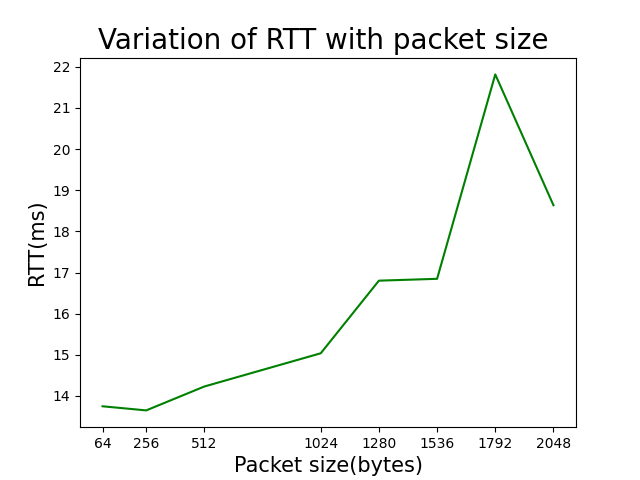
\includegraphics[height=36mm,width=50mm]{ll}
    \hspace{180mm}\vspace{-30mm}
    \FloatBarrier
    \begin{table}[h]
    	\begin{tabular}{c|c|c|c|c|c|c|c|c|}
    		\hspace{55mm}\textbf{Packet size(bytes)}&64&256&512&1024&1280&1536&1792&2048\\
    		\hspace{55mm}\textbf{RTT(ms)}&13.75&13.65&14.23&15.03&16.80&16.84&21.81&18.63\\
    	\end{tabular}
    \end{table}
    \FloatBarrier
    \vspace{15mm}
    \item The data shows that the RTT does not vary much till the packet
    size till 1024 bytes and we see a huge jump when the between 1536 and 1792(RTT almost doubles).The \textbf{MTU i.e the Maximum Transmission unit} is by default 1500 Bytes.If the packet size is less than 1500 the packets are padded to make their size 1500 bytes hence RTT is more or less similar for packets with size less than 1500 Bytes.If the packet size if greater than 1500 Bytes then the packet is broken into two new frames of size 1500 Bytes each and hence we observe almost twice the RTT.
\end{enumerate}
\pagebreak
\section*{Question 3}
\begin{enumerate}[itemsep=-3pt,label=(\alph*)]
	\item Used \textcolor[RGB]{23,0,229}{\textbf{sprinklr.com}} as the host. Packet loss rate in the first case i.e \textbf{-n} is 0\% whereas in other case i.e. \textbf{-p ff00} it is 0.1\%.
	\\ \vspace{-3.5mm}
	\item \begin{tabular}{|c|c|c|c|c|}
		\hline
		\rowcolor[RGB]{0, 145, 255}
		\hspace{1.5mm}\textbf{Command}\hspace{1.5mm}&\hspace{1.5mm}\textbf{Min latency}\hspace{1.5mm} & \hspace{1.5mm}\textbf{Max latency}\hspace{1.5mm} & \hspace{1.5mm}\textbf{Mean latency}\hspace{1.5mm} &\hspace{1.5mm} \textbf{Median latency}\hspace{1.5mm} \\
		\hline
		\rowcolor[RGB]{230, 242, 255}
		ping -n \verb|<IPAddress>| &9.78 ms & 484 ms & 25.604 ms &13.3 ms
		\\ \hline
		
		%252 362 253.689 252.0 8.483058351797423
		%251 751 292.172 281.0 45.81111672945771
		
		\rowcolor[RGB]{0, 247, 255}
		ping -p ff00 \verb|<IPAddress>| &9.23 ms & 176 ms & 25.608 ms &13.2 ms
		\\ \hline
	\end{tabular}\\ \\
    \item 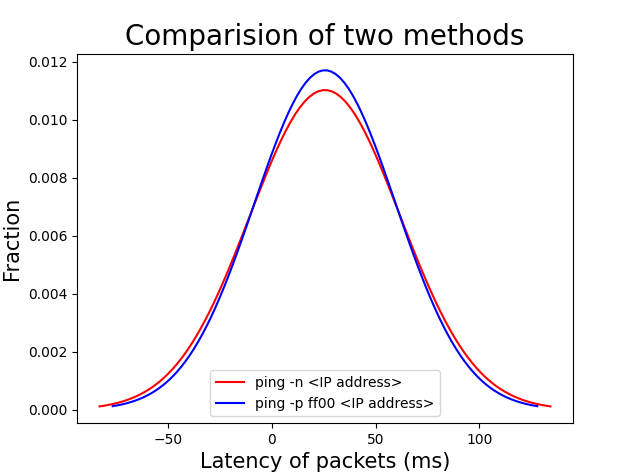
\includegraphics[width=60mm, height=40mm]{comp} 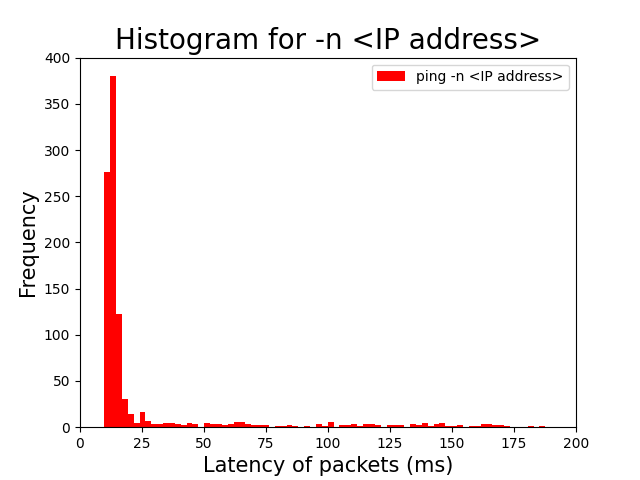
\includegraphics[width=60mm, height=40mm]{1} 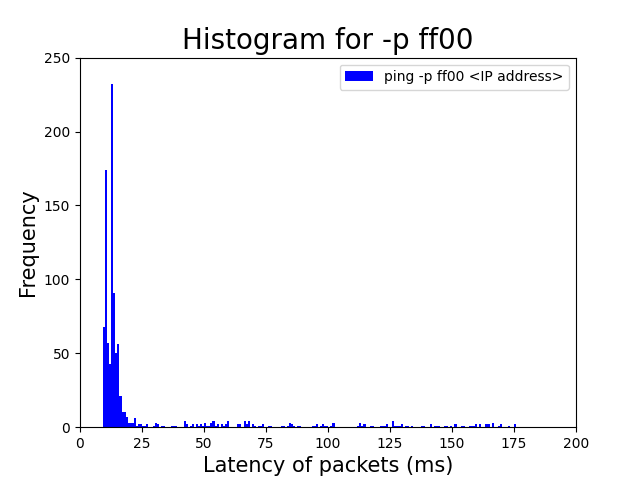
\includegraphics[width=60mm, height=40mm]{2}\\
    \item The two commands are very similar and both represent a normal distribution of values expect that \textbf{-p ff00} sends the packet filled with 8 ones and then 8 zeros i.e \textbf{11111111100000000} which is used to find out the data dependency issues.This will
    cause problems with the synchronisation of the clocks because only one transition is present in the padding, from 1 to 0. Hence,
    the clocks are more likely to go out of synchronisation in case of \textbf{-p ff00} and hence we get a higher packet loss rate. While in case of \textbf{-n} option no attempt would be made to get the symbolic names for the host address hence mean latency is lower in this case.
\end{enumerate}

\section*{Question 4}
\begin{enumerate}[itemsep=-3pt,label=(\alph*)]
	\item \textbf{ifconfig} : It is a command line for UNIX-like systems tool that allows for diagnosing and configuring network interfaces.
	\\
	\\ 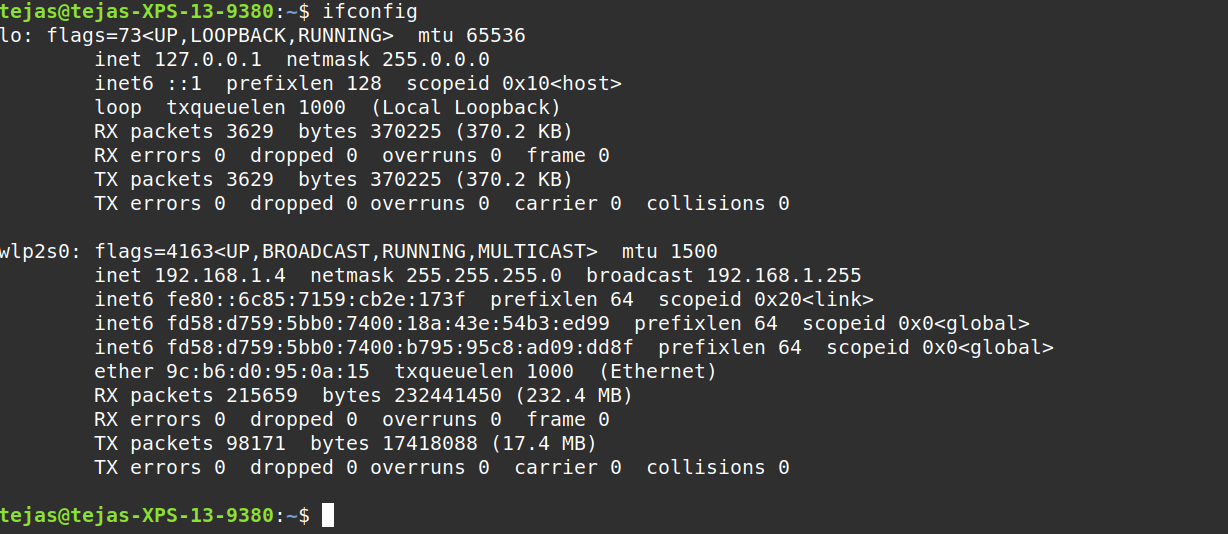
\includegraphics[height=60mm,width=120mm]{config}
	
	\textbf{Network interface} : It is a software interface to networking hardware.Linux kernel distinguishes between two types of network interfaces i.e physical and virtual.
	\vspace{-3mm}
	\begin{enumerate}[itemsep=0pt,label=(\roman*)]
	\item \textbf{Physical network interface} : It represents the actual network hardware such as network interface controller (NIC).
	In practice found \textbf{wlp2s0} interface in the output which represents:\\
	\textbf{wl} for wireless lan (Had it been \textbf{en} instead of \textbf{wl} then \textbf{en} for ethernet) \\The following code is often a description of the physical placement of the device in your computer : \\ \textbf{p2} is likely PCI bus 2 \\ \textbf{s0} is likely slot 0
	\item \textbf{Virtual network interface} : It doesn’t represent any hardware device and is usually linked to one. There are different kinds of virtual interfaces: Loopback (lo), bridges, VLANs, tunnel interfaces etc.Found \textbf{lo i.e Loopback in the output}.
    \end{enumerate}\vspace{-2mm}
%\pagebreak
    \textbf{Interface details}:\vspace{-2mm}
    \begin{enumerate}[itemsep=0pt,label=(\roman*)]
    	\item \textbf{UP}: Indicates that the kernel modules related to the interface have been loaded and interface is activated.
    	\item \textbf{BROADCAST}: Indicates that the interface is configured to handle broadcast packets,which are required for obtaining IP address via DHCP.
    	\item \textbf{RUNNING}: Indicates that the interface is ready to accept the data.
    	\item \textbf{MULTICAST}: Indicates that the interface supports multicasting.
    	\item \textbf{broadcast}: broadcast address for the interface.
    	\item \textbf{netmask}: network mask for the interface.
    	\item \textbf{inet}: IPv4 address assigned to the interface.
    	\item \textbf{inet6}: IPv6 address assigned to the interface.
    	\item \textbf{scope}: It is the scope of IPv6 address. It can be link-local or global.Link-local address is used in local area network and is not routable. Global address is routable.
    	\item \textbf{mtu}: It is the maximum transmission unit.
    \end{enumerate}
     \textbf{Interface stats}:\vspace{-2mm}
     \begin{enumerate}[itemsep=0pt,label=(\roman*)]
     	\item \textbf{RX packets}: The total number of packets received.
     	\item \textbf{RX bytes}: The total number of bytes received.
     	\item \textbf{RX error}: The total number of packets received with errors.
     	\item \textbf{RX dropped}: The total number of number of dropped packets due to unintended VLAN tags or receiving IPv6 frames when interface is not configured for IPv6.
     	\item \textbf{RX overruns}: The number of packets received that experienced fifo overruns, caused by rate at which a buffer gets full and kernel isn’t able to empty it.
     	\item \textbf{RX frame}: The number of of misaligned frames, i.e. frames with length not divisible by 8.
     	\item \textbf{TX packets}: The total number of packets transmitted.
     	\item \textbf{TX bytes}: The total number of bytes transmitted.
     	\item \textbf{TX errors}, \textbf{TX dropped}, \textbf{TX overruns} are similar to RX equivalents.
     	\item \textbf{TX txqueulen}: The length of transmission queue.
     	\item \textbf{TX carriers}: The number of packets that experienced loss of carriers.
     	\item \textbf{TX collisions}: The number of transmitted packets that experienced Ethernet collisions.
     \end{enumerate}
     \item The options which can be used with ifconfig are :\vspace{-2mm}
         \begin{enumerate}[itemsep=0pt,label=(\roman*)]
         	\item \textbf{-s}: This option is used to display short list instead of deatils.
         	\item \textbf{-a}: This option is used to display all the interfaces available even if they are down.
         	\item \textbf{up}: This option is used to activate driver for the given interface.
         	\item \textbf{down}: This option is used to deactivate driver for the given interface.
         \end{enumerate}
     \item The output of route command is organised in the form of a table with following columns:\vspace{-2mm}
          \begin{enumerate}[itemsep=0pt,label=(\roman*)]
          	\item \textbf{Destination}: The destination network or destination host.
          	\item \textbf{Gateway}: The gateway address or ’*’ if none set.
          	\item \textbf{Genmask}: The netmask for the destination net, 255.255.255.255 for a host destination and 0.0.0.0 for the default route.
          	\item \textbf{Flags}:\vspace{-1mm}
          	\begin{enumerate}[itemsep=0pt,label=(\arabic*)]
          		\item U : route is up
          		\item H : target is host 
          		\item G : Use gateway 
          		\item R : reinstate route for dynamic routing
          		\item D : dynamically installed by daemon or redirect 
          		\item M : modified from routing daemon or redirect
          		\item A : installed by addrconf 
          		\item C : cache entry 
          		\item ! : reject route
            \end{enumerate}\vspace{0mm} 
          \item \textbf{Metric}: The distance to the target (usually counted in hops).
          \item \textbf{Ref}: Number of references to this route.
          \item \textbf{Use}: Count of lookups for the route. 
          \item \textbf{Iface}: Interface to which packets for this route will be sent.
          \end{enumerate}
      \item The options which can be used with route command are :\vspace{-2mm}
      \begin{enumerate}[itemsep=0pt,label=(\roman*)]
      	\item \textbf{-n}: This option is used to display routing table in full numeric form and does not resolve names.
      	\item \textbf{-C}: This option is used to display routing cache.
      	\item \textbf{-F}: This option is used to display Forwarding Information Base.
      	\item \textbf{-e}: This option is used to display other/more information.\\
      	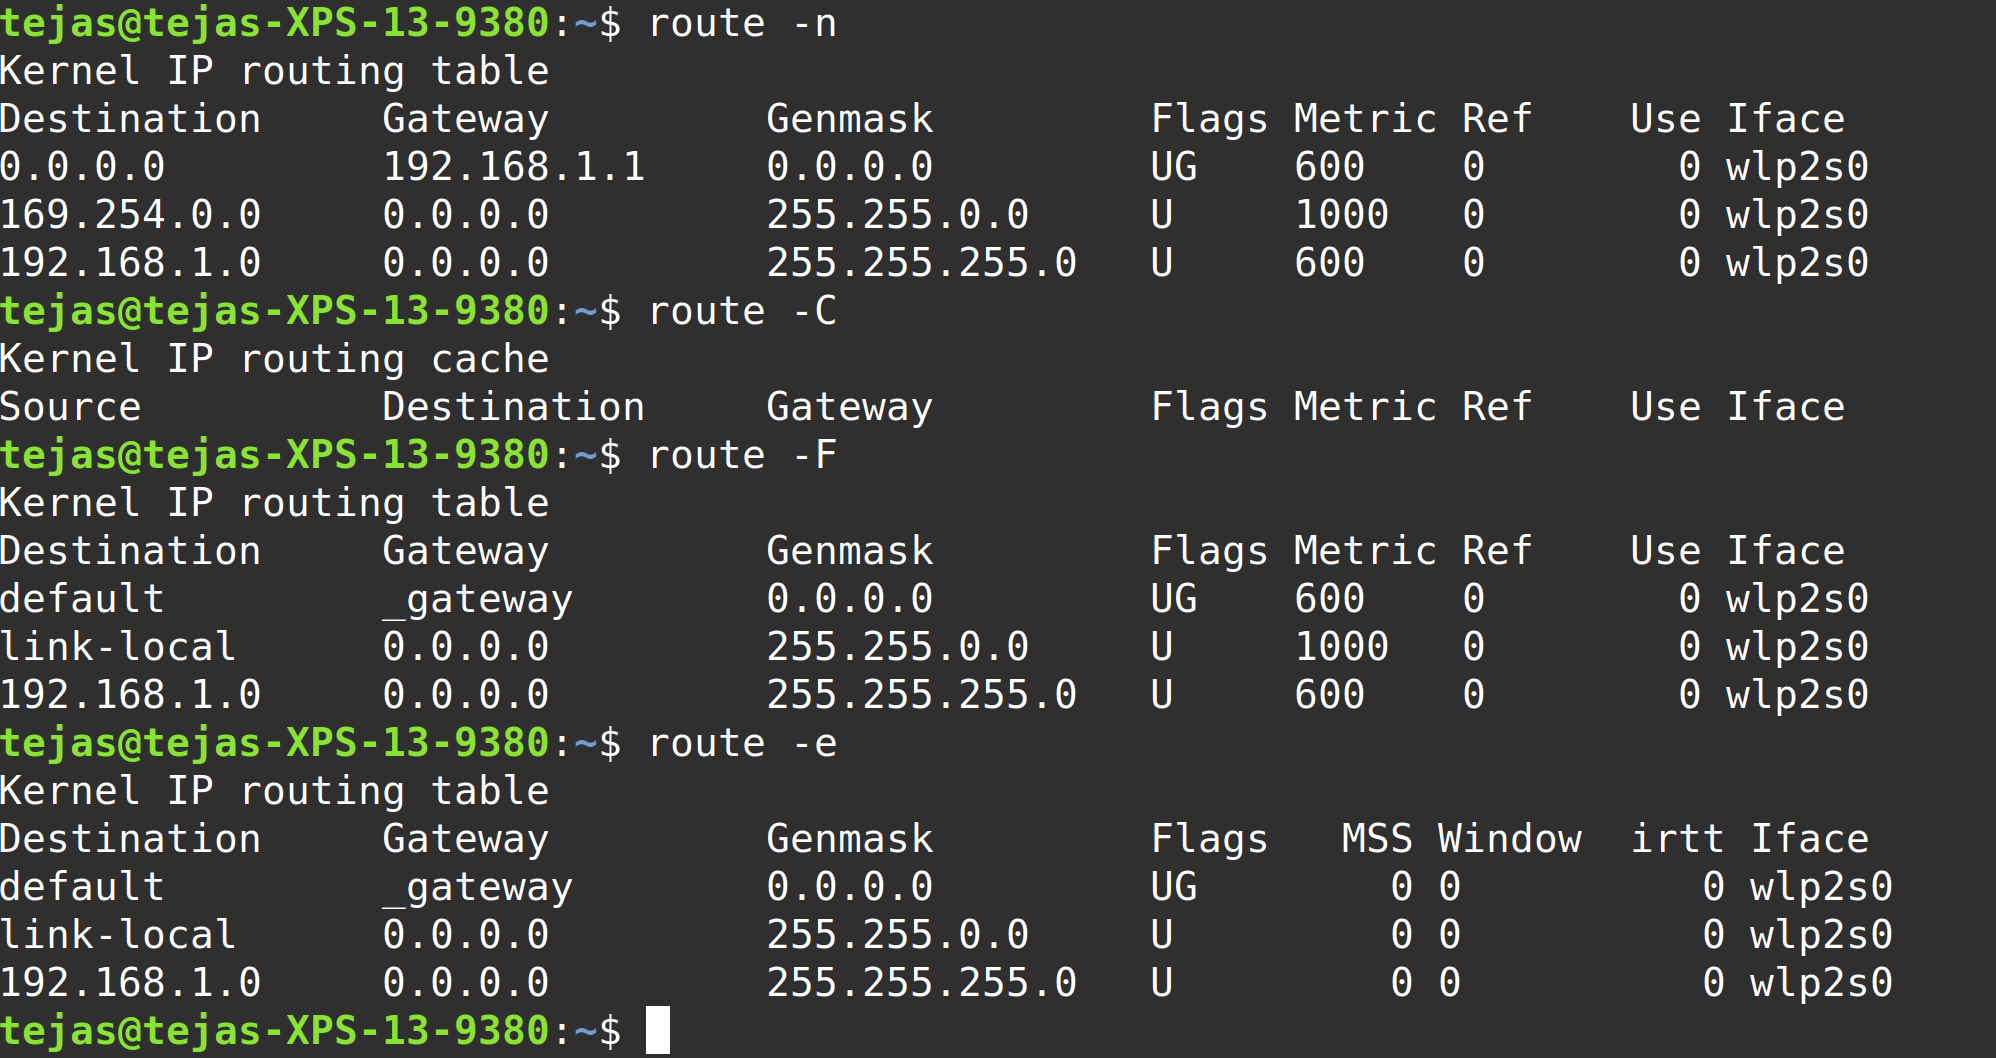
\includegraphics[height=60mm,width=120mm]{route}
      \end{enumerate}
     
\end{enumerate}

\section*{Question 5}
\begin{enumerate}[itemsep=-3pt,label=(\alph*)]
	\item \textbf{netstat (network statistics)} is used for displaying network connections (both incoming and outgoing), routing tables, interface statistics,multicast memberships, masquerade connections. 
	\item netstat -at $|$ grep -n "ESTABLISHED"\\
	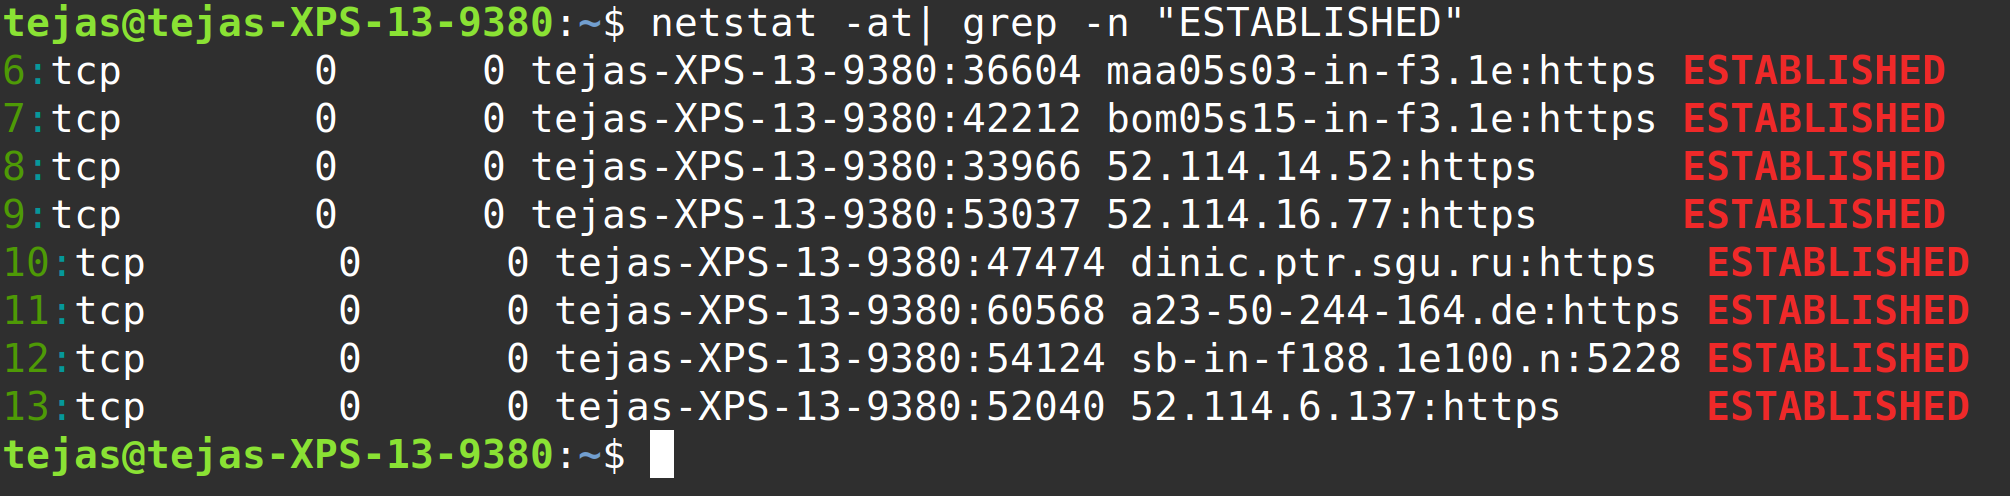
\includegraphics[height=35mm,width=120mm]{tcp_net}
	\item \textbf{netstat -r} shows the kernel routing informations.\\
	The output of the above command is organised in the form of a table with following columns:\vspace{-2mm}
	\begin{enumerate}[itemsep=0pt,label=(\roman*)]
		\item \textbf{Destination}: The destination network or destination host.
		\item \textbf{Gateway}: The gateway address or ’*’ if none set.
		\item \textbf{Genmask}: The netmask for the destination net, 255.255.255.255 for a host destination and 0.0.0.0 for the default route.
		\item \textbf{Flags}:\vspace{-1mm}
		\begin{enumerate}[itemsep=0pt,label=(\arabic*)]
			\item U : route is up
			\item H : target is host 
			\item G : Use gateway 
			\item R : reinstate route for dynamic routing
			\item D : dynamically installed by daemon or redirect 
			\item M : modified from routing daemon or redirect
			\item A : installed by addrconf 
			\item C : cache entry 
			\item ! : reject route
		\end{enumerate}\vspace{0mm} 
	    \item \textbf{MSS}: Default maximum segment size for TCP connections over this route.
	    \item \textbf{Window}: Default window size for TCP connections over this route.
	    \item \textbf{irtt}: Initial RTT(Round trip time).The kernel uses this to guess about the best TCP protocol parameters without waiting on (possibly slow) answers.
		\item \textbf{Iface}: Interface to which packets for this route will be sent.
	\end{enumerate}
	\item The option \textbf{-ai} displays the status of all network interfaces.\\
	The number of interfaces can be found using the command:\\
	\textcolor[RGB]{23,0,229}{echo \$[\$(netstat -ai$|$ wc -l)-2]}\\
	The above command works as all the network interfaces are displayed in the form a table where the first line of the output is the table name and the second line is the names of the columns of the table, Hence the number of interfaces are \textbf{number of lines in the output - 2}.
	\item The option \textbf{-asu} displays the statistics of all the UDP connections.\\
	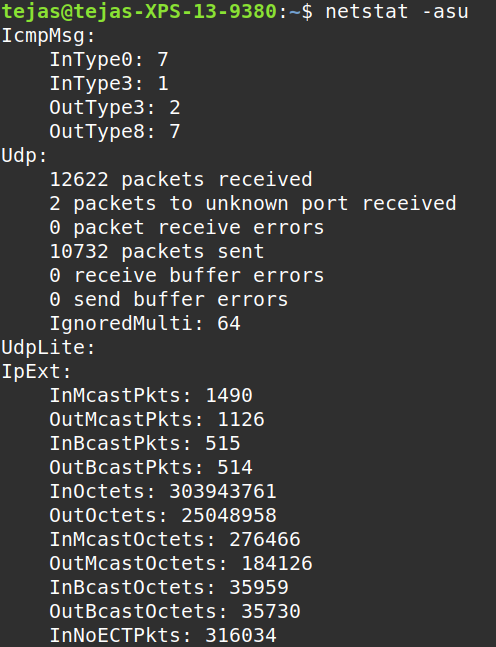
\includegraphics[height=60mm,width=50mm]{udp}
	\item Loopback interface is a virtual interface used by machine to communicate with itself.It is the very first interface to be activated.Occasionally, you will also see the dummy hostname localhost being used instead of the IP-address.Its primary purpose is \textbf{network diagnosis and troubleshooting}.The loopback interface never goes down and provides a \textbf{virtual interface} which is not associated with any hardware.
	When a network interface in a machine is not established, the interface is unable to communicate with the servers in the same machine as well this problem is solved by loopback interface.\\For example you can examine all the web documents that are present on your web server and could examine them file by file on the local machine. For IPv4, the loopback interface is assigned all the IPs in the 127.0.0.0/8 address block i.e 127.0.0.1 - 127.255.255.254.
	
	
\end{enumerate}

\section*{Question 6}
\begin{enumerate}[itemsep=-3pt,label=(\alph*)]
	\item Traceroute is a network diagnostic tool used to track in real-time the pathway taken by a packet on an IP network from source to destination, reporting the IP addresses of all the routers it pinged in between. Traceroute also records the time taken for each hop the packet makes during its route to the destination.
	\item \begin{tabular}{|c|c|c|c|c|}
		\hline
		\rowcolor[RGB]{0, 145, 255}
		\textbf{Sr. no}&\textbf{Host} &\textbf{ Hops @2pm } & \textbf { Hops @8pm }\hspace{0.1mm} & \textbf{ Hops @2am }\\
		\hline
		
			\rowcolor[RGB]{230, 242, 255}
		1&youtube.com & 12 & 12 & 12
		\\ \hline
		
		 \rowcolor[RGB]{0, 247, 255}
		2&codeforces.com & timed out& timed out &timed out 
		\\ \hline
		
			\rowcolor[RGB]{230, 242, 255}
		3&amazon.com & timed out & timed out & timed out 
		\\ \hline
		
			\rowcolor[RGB]{0, 247, 255}
		4&sprinklr.com & 13 & 13 &13
		\\ \hline
		
			\rowcolor[RGB]{230, 242, 255}
		5&facebook.com & 8 & 8 & 8
		\\ \hline
		
		   \rowcolor[RGB]{0, 247, 255}
		6&cricbuzz.com & 16 & 15 &16
		\\ \hline
	\end{tabular}
    \\There were some obvious common hops i.e my device (192.168.1.1) and the IP address of the destination in every case. Apart form that IP address (122.170.255.255) and IP address (122.185.150.53) were the common hops in all the cases as they were the IP addresses of my wifi service provider.If the routes to the destinations pass through the same internet circles then we have common hops.
	\item The route to the hosts changes at different times of the day in the experiments because of network congestion. The packets are redirected by the nodes to take a route having less traffic. The load balancing is done to reduce the load of congested path.
	
	\item Sometimes, traceroute might not find a complete path to some host. Some servers/hosts along the path may have not been configured to respond to the ICMP Traffic or may have set up firewalls which block the ICMP Traffic. However, they still send the data to the next hop as there are results that follow. Moreover,when under heavy load many network providers disable ICMP traffic.
	
	\item It is possible to find the route to certain hosts which fail to respond with ping experiment.Both ping and traceroute use the ICMP Packets but there working is different.
	\\Each IP packet sent on the Internet has a field known as Time-To-Live (TTL). But this field is not explicitly related to the time measured by the number of hops. It is instead, the maximum number of hops that a packet can travel across the Internet before it gets discarded.\\Ping is straight ICMP from point A to point B and has a default TTL value between 1 to 255 which decrements by 1 at every router between the source to destination and expects a \textbf{ICMP Reply Packet} from the host. Most probably the server is blocking the reply.\\ On the other hand, In a traceroute, the source re-defines the TTL value every time it gets a response and sends the packet with TTL=TTL+1 until it reaches its destination.When a packet reaches its maximum TTL, the last hop in line will send back an \textbf{ICMP TTL Exceeded} packet back to the source.\\ Traceroute looks for the ICMP Time exceeded packet and not the ICMP Reply Packet, and that is why it might be possible.
	
	
\end{enumerate}

\section*{Question 7}
\begin{enumerate}[itemsep=-3pt,label=(\alph*)]
	\item \textbf{arp} is used to display the complete ARP table on our machine.
	The output of the above command is organised in the form of a table with following columns:\vspace{-2mm}
	\begin{enumerate}[itemsep=0pt,label=(\roman*)]
		\item \textbf{Hostname}: It is the hostname is the hostname cannot be resolved then you get a ?.
		\item \textbf{IP address}: It is the IP address of the host.
		\item \textbf{MAC address}: It is a six part hexadecimal number. In practice also known hardware address or ethernet address.
		\item \textbf{HWtype}: It is the Hardware type it could be ether i.e ethernet.
		\item \textbf{Flags}:\vspace{-1mm}
		\begin{enumerate}[itemsep=0pt,label=(\arabic*)]
			\item C : Complete Entry
			\item M : Permanent Entry
			\item P : Published Entry
		\end{enumerate}\vspace{0mm} 
	    \item \textbf{Iface}: Network interface.
	\end{enumerate}
    \item \textbf{Delete a entry}: sudo arp -d \verb|<IP address>|\\
    \textbf{Add a entry}: sudo arp -s \verb|<IP address> <MAC address>|
	\\ 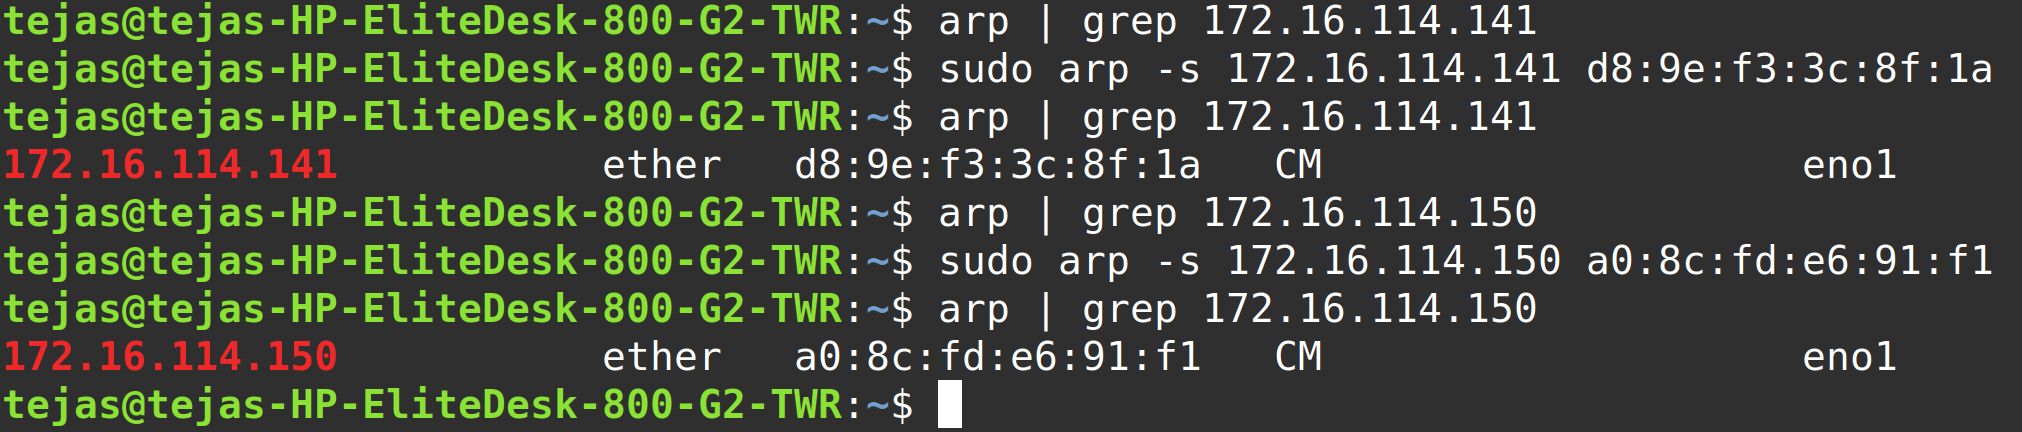
\includegraphics[height=25mm,width=100mm]{arp}
	\item ARP works only when the devices are in the same IP subnet.
	When a device with IP address X needs to send a packet to device with IP address Y , it checks with the routing table whether IP address Y belongs to a subnet it can directly reach through its network interfaces, if this is not the case then device with IP address X uses ARP to map IP address Y to a physical ethernet address and then sends Ethernet frame to that address.\\
	When the two IP addresses are on different subnets, the device will follow a completely different logic i.e. it would check its routing table for a route to the destination network and then it will send its packet to the appropriate router in such a case the ARP will be used to find the hardware address of the router, because the destination IP address ,so the packet must be delivered to a router which can take care of it.
	\item We see a 100\% packet loss when we ping the IP address (say A) whose ethernet address was replaced and 0\% packet loss with the IP address (say B) whose ethernet address was not changed .
	%\\ 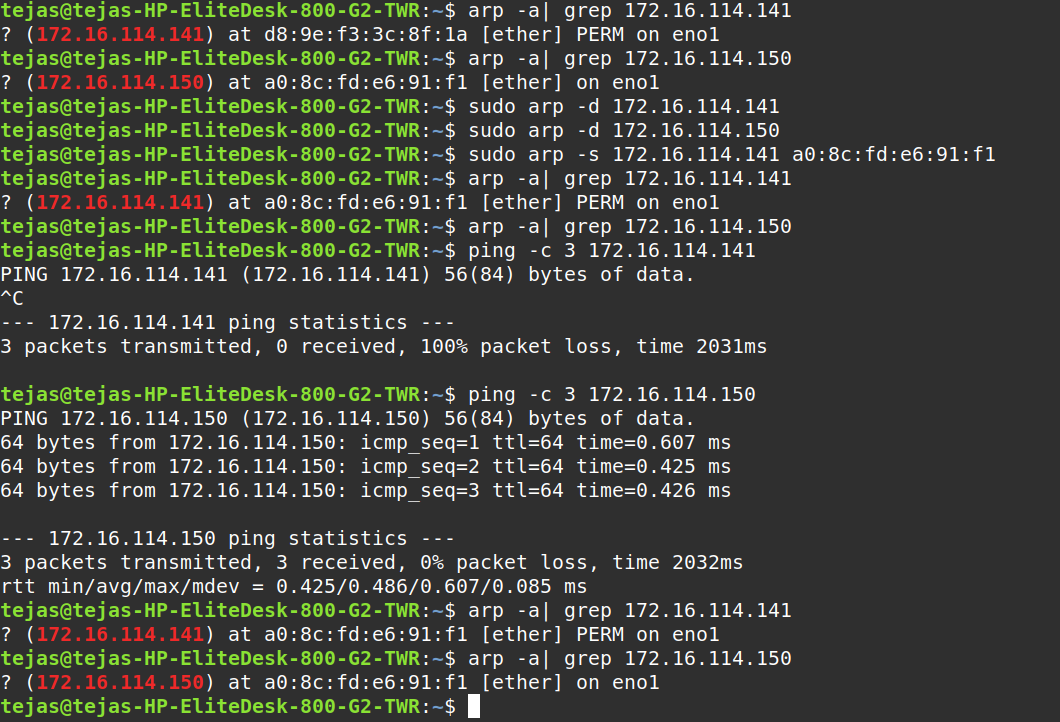
\includegraphics[height=80mm,width=130mm]{arpp}\\
	This happens because IP address A tries to connect through a port which is already occupied and is unable to establish a connection.This results in IP address A being unreachable form other devices in the subnet hence the ping has 100\% packet loss in case of IP address A. 
\end{enumerate}

\section*{Question 8}
\begin{enumerate}[itemsep=-3pt,label=(\alph*)]
	\item nmap -sn \verb|172.16.114.0/24|
	\item nmap -sA \verb|<IP address>|
	\item 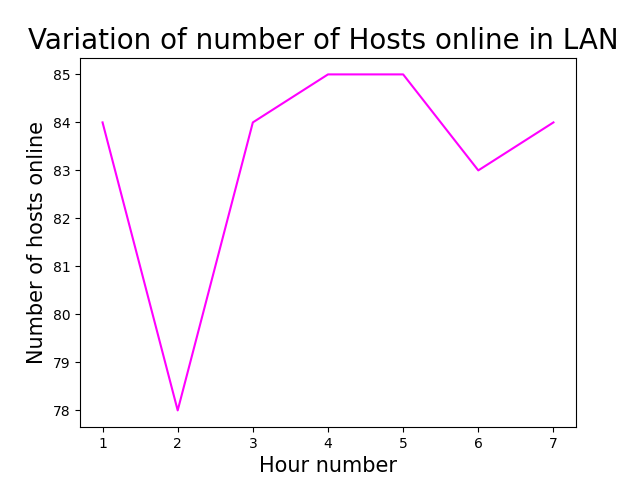
\includegraphics[height=40mm,width=60mm]{host}
	\hspace{180mm}\vspace{-40mm}
	\FloatBarrier
	\begin{table}[h]
		\begin{tabular}{c|c|c|c|c|c|c|c|}
			\hspace{75mm}\textbf{Hour number}&1&2&3&4&5&6&7\\
			\hspace{75mm}\textbf{Hosts online}&84&78&84&85&85&83&84\\
		\end{tabular}
	\end{table}
	\FloatBarrier
	\hspace{66mm} We can observe that the number of hosts that are online at a\\ \phantom{x}\hspace{66mm}given hour is always between 78 and 85.
\end{enumerate}
%172.16.114.141           ether   d8:9e:f3:3c:8f:1a   CM                    eno1
%172.16.114.150           ether   a0:8c:fd:e6:91:f1   CM                    eno1


\end{document}
